%File: formatting-instruction.tex

\documentclass[letterpaper]{article}
\usepackage{aaai16}
\usepackage{times}
\usepackage{helvet}
\usepackage{courier}
\usepackage{graphicx}
\usepackage{subcaption}
\frenchspacing
\setlength{\pdfpagewidth}{8.5in}
\setlength{\pdfpageheight}{11in}

%\documentclass{aamas2013}
\usepackage{amsfonts}
\usepackage{amsmath}
\usepackage{algorithmicx}
\usepackage{algpseudocode}
\usepackage{algorithm}

%\fontsize{24}{6}
%\selectfont


%\usepackage[usenames]{color}
\DeclareMathOperator*{\argmin}{argmin}

%\makeatletter
%\let\@copyrightspace\relax
%\makeatother

% if you are using PDF LaTex and you cannot find a way for producing
% letter, the following explicit settings may help

%\pdfpagewidth=8.5truein
%\pdfpageheight=11truein

\begin{document}


%\TitleForCitationInfo{Robust Learning from Demonstration Techniques and Tools}

\title{Robust Learning from Demonstration Techniques and Tools}

\pdfinfo{
  /Title (Robust Learning from Demonstration Techniques and Tools)
  /Author (William Curran)}

\author{William Curran \\
Oregon State University \\
Corvallis, Oregon \\
curranw@oregonstate.edu \\
%\And
%Adrian Agogino \\
%NASA AMES Research Center \\
%Moffet Field, California \\
%adrian.k.agogino@nasa.gov \\
%\And 
%Kagan Tumer \\
%Oregon State University \\
%Corvallis, Oregon \\
%kagan.tumer@oregonstate.edu \\
}

\maketitle


\begin{abstract}
Large state spaces and the curse of dimensionality contribute to the complexity of a task. Learning from demonstration techniques can be combined with reinforcement learning to narrow the exploration space of an agent, but require consistent and accurate demonstrations, as well as the state-action pairs for an entire demonstration. Individuals with severe motor disabilities are often slow and prone to human errors in demonstrations while teaching. My dissertation develops tools to allow persons with severe motor disabilities, and individuals in general, to train these systems. To handle these large state spaces as well as human error, we developed Dimensionality Reduced Reinforcement Learning. To accommodate slower feedback, we will develop a movie-reel style learning from demonstration interface. 
\end{abstract}


\section{Introduction}
The main goal of my dissertation is to help put robots into real homes to help those with severe physical disabilities. Some
individuals have minimal ability to move and speak, and need extended care all day, every day. The strain on families needing to take care of these individuals is enormous. Inexperienced family caregivers use prescription drugs for depression, anxiety, and insomnia two to three times more often than the average population \cite{Gallagher01081989}. Robotics can be used to assist those with extreme disabilities and remove much of this burden on the family.

These individuals with disabilities are often non-experts, and currently cannot be part of the development process. Yet, most don't want to wait for someone to program autonomous behaviors for all household tasks. We propose to give disabled non-expert users the tools to teach robots tasks by themselves. This will give the disabled user both independence and personal customization.

There are two key difficulties with learning from demonstration interfaces for individuals with disabilities; resolving these are the key contributions of my dissertation. State-of-the-art personal robots need to perform complex manipulation tasks to be viable in assistive scenarios. These complex robots lead to large dimensional state spaces. Also, the ability to perform good demonstrations and give timely feedback are key assumptions in learning from demonstration research \cite{Argall:2009:SRL:1523530.1524008}. My dissertation addresses these assumptions.

The PR2 robot has two 7 DoF arms. When learning position, velocity, and acceleration control, this leads to a 21 dimensional state space per arm. Learning in these high-dimensional spaces is computationally intractable without approximation techniques.  My dissertation introduces Dimensionality Reduced Reinforcement Learning (DRRL) to speed up learning in high-dimensional spaces. DRRL uses demonstrations to compute a projection to a low-dimensional manifold.  In each learning iteration, we project the current state onto this manifold, compute and execute an action, project the new state onto the manifold, and perform a reinforcement learning update. This reduces the number of demonstrations and increases the resistance to suboptimal outliers. These are desirable characteristics in general, but especially for non-expert use of the learning algorithm.

Additionally, we plan to develop a movie-reel style interface for detailed, time-insensitive feedback. This gives the user as much time as they need for demonstrations and feedback.

%\section{Related Work}

%\citeauthor{Grzes::mixed} \shortcite{Grzes::mixed} showed that mixed resolution function approximation works well in complex domains. They build a function approximator that contains a coarse and fine-grained representation, and learn both in parallel. They quickly learn a good function approximation, and over time learn using a more expressive approximation to learn a better quality policy.

%Developing a trajectory using traditional reinforcement learning does not work well in robotics. Finding an optimal or near-optimal solution requires exploration throughout much of the state space. Excessive exploring of the unknown state space risks damaging the robot. Small steps during exploration avoids this problem, but this brings the additional problem of taking longer to find an optimal solution. Initializing, or bootstrapping, the trajectory close to the desired robot behavior removes many of these problems. One approach to this initialization is learning from demonstration.

%One current learning from demonstration research focus is on generalizing motor skills to similar tasks. Pastor et al. uses dynamic motor primitives to perform movement generation and generalization to a new goal \cite{Pastor_ICRA_2009}. However, this approach does not work well with uncertainty. Lee et al. developed belief space learning from demonstration techniques, taking into account uncertainty during learning \cite{Leeetal_IROS2013}. In current research, learning from demonstration requires the human teacher to map their movement directly to the joint angles of the robot and assumes an able-bodied user \cite{Bagnell_2013_7451}.

\section{Learning from Demonstration in High-Dimensional Spaces}
\label{Dimensionality Reduced Reinforcement Learning}

To handle high-dimensional spaces, we performed dimensionality reduction on a set of demonstrated trajectories. We used these demonstrations to compute a projection to a low-dimensional manifold. In each learning iteration, we projected the current state onto this manifold, computed and executed an action, projected the new state onto the manifold, and performed a reinforcement learning update.

We have shown that an agent can learn quickly in the low-dimensional manifold. However, this led to a critical trade-off. By projecting onto a low-dimensional manifold, we discarded low variance, yet potentially important data. By adding DRRL to an existing algorithm, we showed that the agent can quickly converge to a good, yet suboptimal, policy much faster. 

We extended DRRL to add an iterative component (IDRRL). Instead of learning entirely in one manifold, we iteratively learned in all manifolds by using transfer learning. The agent can quickly learn in a low-dimensional space $d$, and transfer that knowledge to the $d+1$ dimensional space using the known mapping between the spaces. We have shown the speed and robustness of this approach when combined with standard Q-Learning in the Mountaincar 3D (Figure 1) domain using good and bad demonstrations. Increasing the robustness to human error in demonstrations and reducing the number of demonstrations are essential. Since we work with individuals with disabilities, physical demonstrations are difficult, and expect suboptimal demonstrations. Since demonstrations are difficult, fewer demonstrations are also a desirable quality.

We plan to extend this work to robotic control. By parameterizing the motor primitives in a low-dimensional manifold, we hypothesize that we will be able to more easily generalize motor skills to similar tasks.  This will reduce the number of different demonstrations required. Additionally, dimensionality reduction smooths the lower-dimensional trajectory. We hypothesize that this makes the learning more robust to suboptimal outliers caused by human error. 

\begin{figure}[]
  \centering
      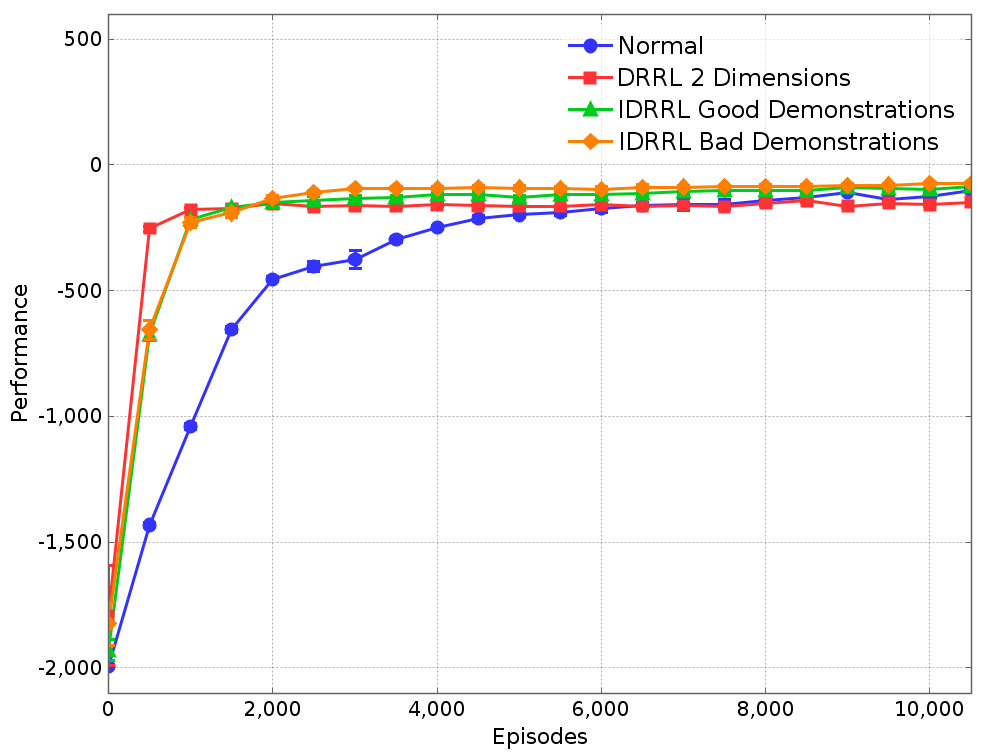
\includegraphics[width=0.38\textwidth]{IDRRL_DC}
  \caption{DRRL and IDRRL were combined with standard Q-Learning. DRRL converged faster, but to a slightly suboptimal solution. IDRRL converged quickly to an optimal solution. Additionally, IDRRL is robust to suboptimal demonstrations in Mountain Car 3D.}
  \label{fig:IDRRL_3DMountainCar}
\end{figure}

\section{Learning from Demonstration Interfaces}
\label{Learning by Demonstration}

We need to develop a learning from demonstration interface that allows individuals with disabilities to teach their assistive robot at their own speed. We propose two interfaces: an early interface for super users, and one for users with severe physical disabilities. In this work we will use RViz, a ROS package that assists users in the visualization of robotic movements and sensors \cite{quigley:ros}.  Our first focus of research is to extend RViz to be an interface for learning from demonstration. 

The interface for users without disabilities will take advantage of the direct first-person control aspect of RViz.  We will also use the Oculus Rift and Razer Hydra control systems. The Oculus Rift allows a user to see through the sensors of the robot, while the Hydra controls the robot. The Hydra control system computes the exact location and orientation of controllers in your hands, allowing the user more natural control of the robotic arms. Using these tools the user can efficiently teach the robot through demonstration.

The interface for users with disabilities will use a less direct approach. The robot will come with a motion library of basic autonomous functions, such as turning knobs and picking up objects. First, the user will give the robot a sequence of these high level actions to perform the task. The robot will simulate itself doing the task in RViz. We will extend RViz with a movie-reel style interface for rewinding and fast forwarding of the robot's simulation. The user can then provide feedback on an action at his or her own speed. This learning from demonstration interface allows the users to build custom routines for the robot without direct knowledge of the reinforcement learning algorithm.

To analyze the initial efficacy of the movie-reel style interface there will be a within-subjects study, in which the users will be able-bodied. We will take objective measurements such as the total task time and the user's cognitive load, as well as subjective measurements with questionnaires. We will then perform another study with disabled individuals that have previously worked with our lab. Comparing the results will give us a better understanding of the efficacy of the interface.


%\section{Evaluation}
 %To analyze our dimensionality reduction research in robotics, we will compare learning speed and efficiency to the dynamic motor primitive work by Pastor et al. \cite{Pastor_ICRA_2009} and the belief state planning by Lee et al. \cite{Leeetal_IROS2013}.

\section{Conclusion}
%Those suffering from ALS and quadriplegia need robots in the world now, and cannot wait for full autonomy of every task. This work intends to help those suffering from severe physical disabilities by giving them the ability to teach the robot themselves, as well as to easily give positive and negative feedback. By using our shared autonomy approach we separate the low-level reactivity from the higher level reasoning, and give the higher-level reasoning task to the user. 

Those suffering from ALS and quadriplegia need assistive robots now. These individuals cannot wait for someone to program autonomous behaviors for all household tasks.  This work intends to help those suffering from severe physical disabilities by giving them the ability to teach the robot themselves.

%This work also helps further the state of the art in reinforcement learning by introducing a new learning from demonstration technique that utilizes human demonstration from non-experts. This requires robots to learn from human demonstrations, even when those demonstrations are highly suboptimal. By transforming high-dimensional learning from demonstration trajectories to a lower-dimensional space, we hypothesize that we this approach will assist in generalizing between similar tasks, as well as increase the robustness of learning trajectories with suboptimal outliers.

This work introduces a new learning from demonstration technique that utilizes human demonstration from non-experts. This requires robots to learn from human demonstrations, even when those demonstrations are suboptimal. By learning in a lower-dimensional space, we hypothesize that it will be easier to generalize between similar tasks, as well as ease the learning of trajectories with outliers.

%One of the key difficulties of assistive robots is human trust. If humans had constant direct control of the robot, they would be forced to extend a high cognitive load and take a lot of time every situation they wanted the robot to perform a task. With a shared autonomy system, humans perform the high level reasoning, while the robot retains the low level reactivity.

%With these new interfaces and tools, individuals with disabilities will be able to accomplish day-to-day tasks without assistance from others. The lack of a human assistant performing the task and the addition of positive experiences like teaching, doing it yourself, and being more independent increases the quality of life for peoples with extreme disabilities.

With these new interfaces and learning advances, individuals with disabilities will be able to do day-to-day tasks without help from others. The lack of a human assistant performing the task and the addition of positive experiences like teaching, doing it yourself, and being more independent increases the quality of life for people with extreme disabilities.

%Our first avenue of work involves extending RIDE to allow users to easily teach robots through demonstration. The two interfaces we develop will give us insight on how to design a remote learning by demonstration system for users with and without disabilities. This interface will allow users to be able to teach robots how to perform tasks around their home easily and efficiently.

%We will combine the learning by demonstration interface with a Google Glass object classification system. This Google Glass system will allow users to add semantic information to objects within their home. This semantic information can be sent to the robot wirelessly, and used when given tasks.

%Lastly, we will extend this work for multi-robot interaction. By extending RIDE to become task-based, users will be able to give high level tasks to one or many robots, applying the previously learned behavior and semantic mappings. This interface will be able to be used via Google Glass, for hands-free task allocation.


\bibliographystyle{aaai}
\bibliography{thesis}

\end{document}
